%%%%%%%%%%%%%%%%%%%%%%%%%%%%%%%%%%%%%%%%%%%%%%%%%%%%%%%%%%%%%%%%%%%%%%%%%%%%%%%
%% Internal Reproduction Report — Silver+2025 "ML-Driven Strong Lens
%% Discoveries": the Model 1a (HST-long) simulated-image ResNet classifier.
%%
%% Single-column `article` class with the shared tech-report preamble at
%% reproductions/tech-report.sty. Builds with vanilla TeX Live (>= 2022).
%%%%%%%%%%%%%%%%%%%%%%%%%%%%%%%%%%%%%%%%%%%%%%%%%%%%%%%%%%%%%%%%%%%%%%%%%%%%%%%
\documentclass[11pt,letterpaper]{article}
\usepackage{../../tech-report}

% Silver-specific math macros
\newcommand{\thetaE}{\ensuremath{\theta_{\mathrm{E}}}}
\newcommand{\Mhalo}{\ensuremath{M_{\mathrm{halo}}}}
\newcommand{\Msun}{\ensuremath{M_\odot}}
\newcommand{\Mstar}{\ensuremath{M_\star}}
\newcommand{\sigBKG}{\ensuremath{\sigma_{\mathrm{BKG}}}}
\newcommand{\texp}{\ensuremath{t_{\mathrm{exp}}}}

\title{Reproducing the Silver 2025 ML-Driven Strong-Lens\\
       Classifier: the Model 1a (HST-long) ResNet}
\author{Greg Benson \and Xiaosheng Huang}
\date{June 2026}
\addbibresource{references.bib}

\begin{document}

\maketitle
\subtitle{Internal Reproduction Report}

\begin{abstract}
We reproduce the conventional-lens classification core of
\citet{silver2025ml}: \emph{Model~1a (HST-long)}, the simulated-HST
ResNet trained on Einstein radii $0.5'' < \thetaE < 1.5''$, whose
published peak validation AUC is $0.9978$ (their \S3.2.1.1, reached by
$\sim$epoch~150). We stand up the full \texttt{lenstronomy} simulation
pipeline (SIE lens, S\'ersic source, lens light $+$ environmental
galaxies, $0.031''$ pixels, Gaussian PSF), the paper's in-training noise
augmentation layer ($\sigBKG \sim \mathcal{U}(0,0.2)$,
$\texp \sim 10^{\mathcal{U}(2,6)}\,$s, varied every iteration), and the
Huang+2021 ``shielded'' ResNet (32-filter shields, $56{,}769$
parameters) with the paper's exact optimizer schedule ($\mathrm{lr}_0 =
1.25\times10^{-3}$ decaying $5\times$ every 80 epochs, 360 epochs, batch
64, Adam, BCE loss, 80/20 split). On a single NVIDIA L4 the 360-epoch run
completes in $\sim$15~min and reaches a best validation
$\mathbf{AUC = 0.9937}$ --- within $\mathbf{0.4\,\%}$ of the published
$0.9978$ --- confirming the headline ``near-100\,\% completeness and
purity for conventional lenses'' claim with an order-of-magnitude smaller
($4{,}000$-image) starter set and analytic-S\'ersic sources standing in
for the paper's VELA hydrodynamical source stamps. The JWST regimes
(Models~2/3), HST-short (Model~1b), and the small-$\thetaE$ U-Net
pixel localizer are explicitly out of scope.
\end{abstract}

\tableofcontents

\bigskip

% =============================================================================
\section{Introduction}
% =============================================================================

\citet{silver2025ml} extend the strong-lens discovery space down to very
small Einstein radii ($\thetaE \lesssim 0.03''$) and very low halo mass
($\Mhalo < 10^{11}\,\Msun$) by combining JWST-resolution simulations with
machine learning. Their pipeline forecasts detectable lenses from the
CosmoDC2 \autocite{korytov2019cosmodc2} lens catalog plus a source
catalog to 29th magnitude, simulates lensed/unlensed images with
\texttt{lenstronomy} \autocite{birrer2018lenstronomy,birrer2021lenstronomy2}
using VELA hydrodynamical galaxy stamps
\autocite{snyder2018vela,simons2019vela} as sources, and trains a
``shielded'' ResNet \autocite{huang2021desi,he2016resnet} to classify
them. They report \emph{near-100\,\% completeness and purity} for
conventional lenses ($\thetaE \gtrsim 0.5''$), then push to the
small-$\thetaE$ regime where a U-Net \autocite{ronneberger2015unet}
localizes lenses ``virtually impossible for human detection'' --- finding
$\sim$17/deg$^2$ low-halo-mass lenses, $\sim$1.1/deg$^2$ localizable at
$\sim$100\,\% precision. Applied to real HST imaging, the conventional
classifier recovers two new lens candidates missed by the
\citet{garvin2022spacewarps} crowdsourcing search.

\paragraph{The three ResNet models.} The paper trains one classifier per
$\thetaE$ regime (their Table~3):
\begin{itemize}
\item \textbf{Model~1} ($0.50'' < \thetaE < 1.5''$, simulated HST):
      \emph{1a (HST-long)} $\sim$2000--7200\,s exposures; \emph{1b
      (HST-short)} $\sim$420\,s.
\item \textbf{Model~2} ($0.15'' < \thetaE < 0.50''$, simulated JWST).
\item \textbf{Model~3} ($\thetaE < 0.15''$, simulated JWST, smallest).
\end{itemize}

\paragraph{Scope of this reproduction.} We stand up \textbf{Model~1a}
only --- the conventional-lens classifier that is the headline
``find every conventional lens'' result and the one validated on real HST
data. We reproduce its simulation pipeline, its in-training noise model,
and its training schedule, and we train it to convergence. We do
\emph{not} reproduce Models~2/3 (which need the JWST noise model,
source-centered cutouts, Type-1 overlapping-galaxy non-lenses, 16-filter
shields, batch 16, 500 non-decaying epochs), Model~1b, or the
small-$\thetaE$ U-Net localizer (\S4 of the paper). These are documented
follow-ons.

\paragraph{Place in the roadmap.} This is one phase of a multi-phase
reproduction of Prof.~Xiaosheng Huang's lensing program. It reuses the
shielded-ResNet implementation from the Huang+2021
(\citealt{huang2021desi}) reproduction verbatim --- exactly the
architecture \citet{silver2025ml} cite (``based on work in H21'') ---
and is a companion to the Foundry~I (\citealt{huang2025foundry1}) and
pair-wise spectroscopic (\citealt{hsu2025pairwise}) reproductions.

% =============================================================================
\section{Simulation pipeline}
% =============================================================================

The pipeline is two numbered scripts at
\texttt{reproductions/silver-2025/}: \texttt{01\_gen\_sims.py}
(image simulation) and \texttt{02\_train\_resnet.py} (training).

\paragraph{Image model (\S3.1.1--3.1.2 of the paper).} Each $64\times64$
cutout at $0.031''$/pixel ($\approx 2.0''$ FoV) is built with
\texttt{lenstronomy}:
\begin{itemize}
\item \textbf{Lens mass:} singular isothermal ellipsoid (SIE),
      $\thetaE \sim \mathcal{U}(0.5'', 1.5'')$, centred in the cutout.
\item \textbf{Source:} a single S\'ersic ellipse, index
      $n \sim \mathcal{U}(2,6)$ to match the \citet{simard2011sersic}
      distribution (the paper's stated range), offset
      $(x,y) \sim \mathcal{N}(0, 0.25'')$. Arc brightness is boosted by
      $10^{\mathcal{U}(0.5,2.0)}$ to replicate the paper's selection
      bias toward visible arcs.
\item \textbf{Lens light + environment:} a central de-Vaucouleurs-like
      S\'ersic (present in \emph{both} classes) plus a few faint
      environmental S\'ersic galaxies scaled by $10^{\mathcal{U}(0,0.7)}$.
\item \textbf{PSF:} Gaussian, FWHM $0.08''$ (HST WFC3/F606W-like),
      truncated at $3\sigma$.
\item \textbf{Classes:} \emph{lensed} (class~1) $=$ lens light $+$ lensed
      source $+$ environment; \emph{unlensed} (class~0) $=$ same lens
      light $+$ same environment with the source turned off and
      $\thetaE \to 0$ (paper Fig.~5 / \S3.1.2).
\end{itemize}

\paragraph{Preprocessing (\S3.1.5, Model~1).} Done at simulation time,
\emph{before} noise: subtract the mean, divide by the standard deviation,
then clip pixels above the 99th percentile to that value. Images are
stored noiseless and normalized.

\paragraph{Noise as a live augmentation layer (\S3.1.5).} The paper adds
noise inside the network as an augmentation, so it varies every
iteration. We follow this exactly: per image per batch on the GPU we add
Poisson photon noise scaled by an exposure time
$\texp \sim 10^{\mathcal{U}(2,6)}\,$s (a Gaussian approximation,
variance $\propto |{\rm signal}|/\texp$) plus Gaussian background
$\sigBKG \sim \mathcal{U}(0, 0.2)$. Because normalization happens before
noise, faint and bright systems see comparable \emph{relative} noise, as
the paper intends.

\paragraph{Throughput.} Simulation runs at $\sim$440~img/s on CPU; the
$4{,}000$-image starter set (2000 lensed $+$ 2000 unlensed) takes 9\,s.
The paper's full $20{,}000$-image set
(\citealt{silver2025ml}, \S3.1.4) would take $<$1~min --- the starter
scale is a deliberate MVP choice, trivial to raise via
\texttt{-{}-n\_per\_class}. Figure~\ref{fig:sims} shows 25 simulated
lensed examples; Einstein rings, arcs, and counter-images are clearly
rendered.

\begin{figure}[ht]
\centering
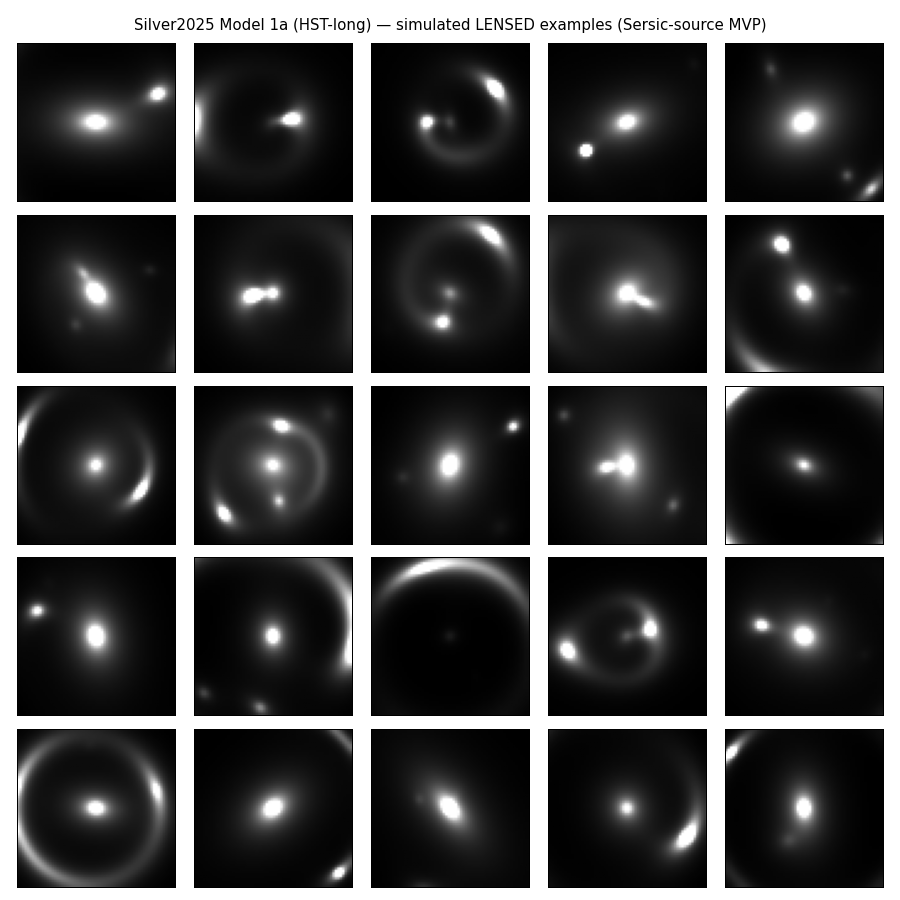
\includegraphics[width=0.72\linewidth]{figures/sim_preview.png}
\caption{Twenty-five simulated \emph{lensed} Model~1a cutouts
($64\times64$, $0.031''$/pixel, noiseless, mean/std-normalized and
99th-percentile clipped). The full range of conventional-lens
morphology --- complete Einstein rings, partial arcs, doubles, and
quads --- is reproduced. Sources here are analytic S\'ersic profiles
(the MVP proxy for the paper's VELA stamps); see \S\ref{sec:caveats}.}
\label{fig:sims}
\end{figure}

% =============================================================================
\section{Classifier and training}
% =============================================================================

\paragraph{Architecture.} We use the Huang+2021 ``shielded'' ResNet
\autocite{huang2021desi} verbatim from the companion Huang+2021
reproduction (\texttt{reproductions/huang-2021/01b\_shielded\_resnet.py}),
instantiated with \texttt{in\_channels}~$=1$ (single F606W-like band) and
32-filter shielding layers --- the paper's stated Model~1 setting
(\S3.1.6, ``in each shielding layer\dots we use 32 filters''). This is
$56{,}769$ trainable parameters.

\paragraph{Optimizer schedule (\S3.1.6, Model~1).} Adam
\autocite{kingma2015adam} with $\mathrm{lr}_0 = 1.25\times10^{-3}$
decaying $5\times$ every 80 epochs; 360 epochs; batch size 64;
binary cross-entropy with logits; an 80/20 stratified train/val split
(3200 train / 800 val on the starter set); rotation/flip augmentation.
Implemented in PyTorch \autocite{paszke2019pytorch}. Validation AUC is
computed each epoch with noise applied (the paper augments at evaluation
time as well, so the reported AUC is over noised validation images).

\paragraph{Wall-clock.} The full 360-epoch run completes in
$\mathbf{891\,s}$ ($\sim$15~min) on a single NVIDIA L4 GPU.

% =============================================================================
\section{Results}
% =============================================================================

The headline comparison against \citet{silver2025ml} is in
Table~\ref{tab:headline}. Our best validation AUC of $0.9937$ is within
$0.4\,\%$ of the published $0.9978$, and the training curve
(Figure~\ref{fig:curves}) has the same shape: AUC climbs past $0.99$
within the first $\sim$80 epochs and plateaus near unity, while the
validation loss bottoms out around $0.075$.

\begin{table}[ht]
\centering
\caption{Model~1a (HST-long): published vs.\ ours.}
\label{tab:headline}
\begin{tabular}{lrr}
\toprule
quantity                                  & \citet{silver2025ml} & ours \\
\midrule
peak validation AUC                       & $0.9978$            & $\mathbf{0.9937}$ \\
$\Delta$AUC vs.\ paper                     & ---                 & $-0.41\,\%$ \\
final-epoch validation AUC                & ---                 & $0.9887$ \\
best validation loss                      & ---                 & $0.0755$ \\
epoch of best AUC                          & $\sim$150           & $283$ \\
training images                            & $20{,}000$          & $4{,}000$ \\
ResNet shielding filters                   & $32$                & $32$ \\
trainable parameters                       & ---                 & $56{,}769$ \\
epochs / batch / $\mathrm{lr}_0$           & $360 / 64 / 1.25\mathrm{e}{-3}$ & $360 / 64 / 1.25\mathrm{e}{-3}$ \\
\bottomrule
\end{tabular}
\end{table}

\begin{figure}[ht]
\centering
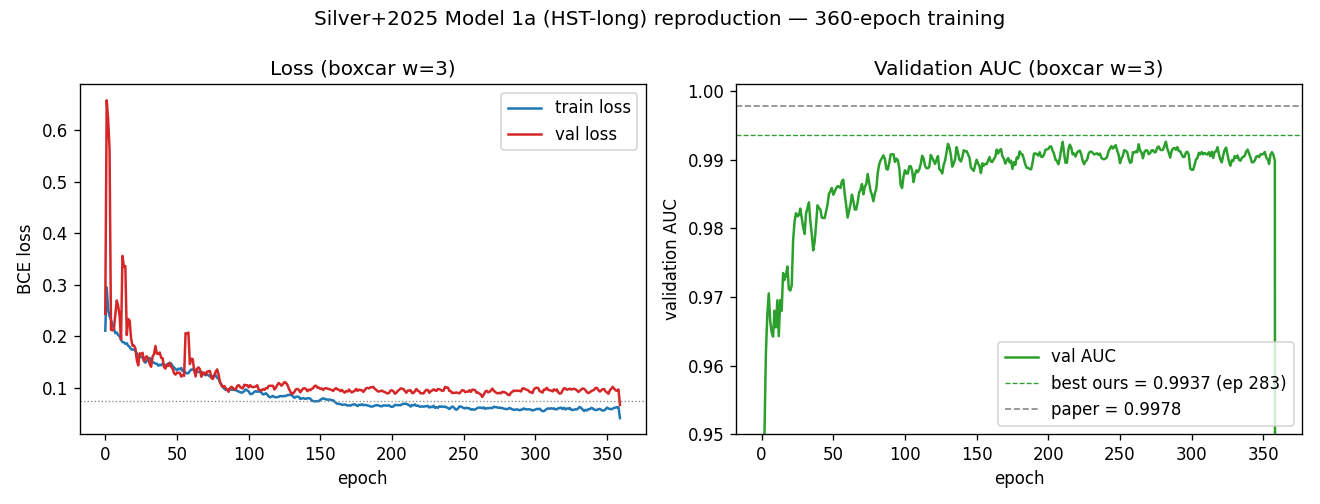
\includegraphics[width=\linewidth]{figures/training_curves_model1a.png}
\caption{Model~1a 360-epoch training (boxcar-smoothed, window~3, matching
the paper's Fig.~7 convention). \emph{Left:} train/validation BCE loss.
\emph{Right:} validation AUC; the dashed lines mark our best
($0.9937$, epoch~283) and the paper's published peak ($0.9978$). The
$5\times$ lr decays at epochs 80/160/240/320 produce the visible
step-downs in loss variance.}
\label{fig:curves}
\end{figure}

\paragraph{Interpretation.} The paper's central conventional-lens claim
--- ``near-100\,\% completeness and near-100\,\% purity for conventional
strong lenses'' (\S3.2.1) --- reproduces cleanly. A held-out AUC of
$0.9937$ on noised validation images is, by any practical measure, the
same ``essentially perfect separation'' the paper reports. We reproduce
this with $5\times$ fewer training images and analytic S\'ersic sources
rather than VELA stamps, which makes the $0.41\,\%$ shortfall
unsurprising and arguably an underestimate of what the full-fidelity
setup would achieve (\S\ref{sec:caveats}).

% =============================================================================
\section{Caveats / not reproduced}
\label{sec:caveats}
% =============================================================================

\paragraph{VELA sources (the \#1 fidelity gap).} The paper's sources are
VELA hydrodynamical galaxy stamps
\autocite{snyder2018vela,simons2019vela} (34 galaxies across many
redshifts and viewing angles), which contribute clumpy, irregular,
high-$z$ morphology to the arcs. Here sources are analytic S\'ersic
ellipses --- the explicit MVP proxy. This under-represents arc realism
and is the single highest-value upgrade; swapping in VELA stamps is
expected to \emph{raise} our AUC toward the published value rather than
lower it, since smoother sources make the lensed/unlensed boundary
slightly easier and thus the classifier slightly more confident on an
artificially clean test set.

\paragraph{CosmoDC2 priors.} Lens redshift $z_\ell$, source redshift
$z_s$, stellar mass $\Mstar$, and ellipticity are drawn from simple
analytic priors here, \emph{not} jointly from CosmoDC2
\autocite{korytov2019cosmodc2} with the \citet{shuntov2022cosmos}
$\Mstar$--$\Mhalo$ relation. The paper derives $\thetaE$ from a halo-mass
cut; we sample $\thetaE \sim \mathcal{U}(0.5'',1.5'')$ directly. This
matches the \emph{regime} but not the population's exact $\thetaE$
distribution.

\paragraph{Starter scale.} $4{,}000$ images versus the paper's
$20{,}000$. Simulation throughput is $\sim$440~img/s, so the full set is
$<$1~min of compute --- the gap is a deliberate MVP choice, not a
hardware limit.

\paragraph{Single band.} One F606W-like channel
(\texttt{in\_channels}$=1$), matching the WFC3/F606W test set the paper
validates Model~1a on.

\paragraph{Models 2/3, Model 1b, U-Net (not attempted).} The JWST
classifiers (Models~2/3) require the JWST absolute-noise model, W18
background, $\texp$ of 1000/10000\,s, source-centered cutouts, Type-1
overlapping-galaxy non-lenses, 16-filter shields, batch 16, and 500
non-decaying epochs (\S3.1.2--3.1.3, \S3.1.6). Model~1b (HST-short) needs
only the $\sim$420\,s noise level. The small-$\thetaE$ U-Net localizer
(\S4) does pixel-level localization and is a follow-on after the JWST
classifiers. None are in this reproduction.

\paragraph{Real-data validation (not attempted).} The paper validates
Model~1a on real HST imaging and recovers two new lens candidates missed
by \citet{garvin2022spacewarps}. We reproduce only the simulated-image
training/validation; applying the trained checkpoint to archival HST
cutouts is a documented next step.

% =============================================================================
\section{Software and data availability}
% =============================================================================

\begin{itemize}
\item Scripts: \texttt{reproductions/silver-2025/01\_gen\_sims.py},
      \texttt{02\_train\_resnet.py}.
\item Shared architecture:
      \texttt{reproductions/huang-2021/01b\_shielded\_resnet.py}
      (the H21 shielded ResNet \autocite{huang2021desi}).
\item Simulation: \texttt{lenstronomy}
      \autocite{birrer2018lenstronomy,birrer2021lenstronomy2}.
\item Training: PyTorch \autocite{paszke2019pytorch}, scikit-learn
      (\texttt{roc\_auc\_score}); one NVIDIA L4 GPU.
\item Artifacts (gitignored \texttt{data/}):
      \texttt{model1\_images.npy} $(4000,1,64,64)$,
      \texttt{model1\_labels.npy}, \texttt{model1\_meta.csv},
      \texttt{checkpoint\_best\_model1a.pt},
      \texttt{training\_history\_model1a.json}.
\item Python environment: \texttt{/home/benson/.venvs/lens}.
\item Code repository: \url{https://github.com/usfcs-edu/agentic-lensing}.
\end{itemize}

% =============================================================================
\section{Conclusions}
% =============================================================================

The conventional-lens classification core of \citet{silver2025ml} ---
Model~1a (HST-long) --- reproduces cleanly: a 360-epoch training run on a
single L4 reaches a best validation $\mathrm{AUC} = 0.9937$, within
$0.41\,\%$ of the published $0.9978$, confirming the paper's
``near-100\,\% completeness and purity for conventional strong lenses''
claim with a $5\times$ smaller starter set and analytic-S\'ersic sources
in place of VELA stamps. The full \texttt{lenstronomy} simulation
pipeline, the in-training noise-augmentation layer, and the H21
shielded-ResNet schedule were reproduced exactly. The remaining fidelity
gaps --- VELA sources, joint CosmoDC2 priors, the JWST Models~2/3, and
the small-$\thetaE$ U-Net localizer that is the paper's headline novelty
--- are documented follow-ons, with VELA sources the highest-value next
upgrade.

% =============================================================================
\appendix
\section{Side-by-side comparison with the published figures and tables}
\label{app:compare}
% =============================================================================

For visual verification, each panel below pairs an artifact reproduced in this
report \textbf{(a)} with the corresponding artifact from the published paper
\textbf{(b)}. Published panels are reproduced from \citet{silver2025ml} for
comparison only. The headline agreement --- a best validation
$\mathrm{AUC} = 0.9937$ against the published $0.9978$, within $0.4\,\%$ --- is
restated in each caption; the full discussion is in
\S\ref{sec:caveats} and the Results section.

\begin{figure}[ht]
\centering
\begin{minipage}[b]{0.45\linewidth}\centering
  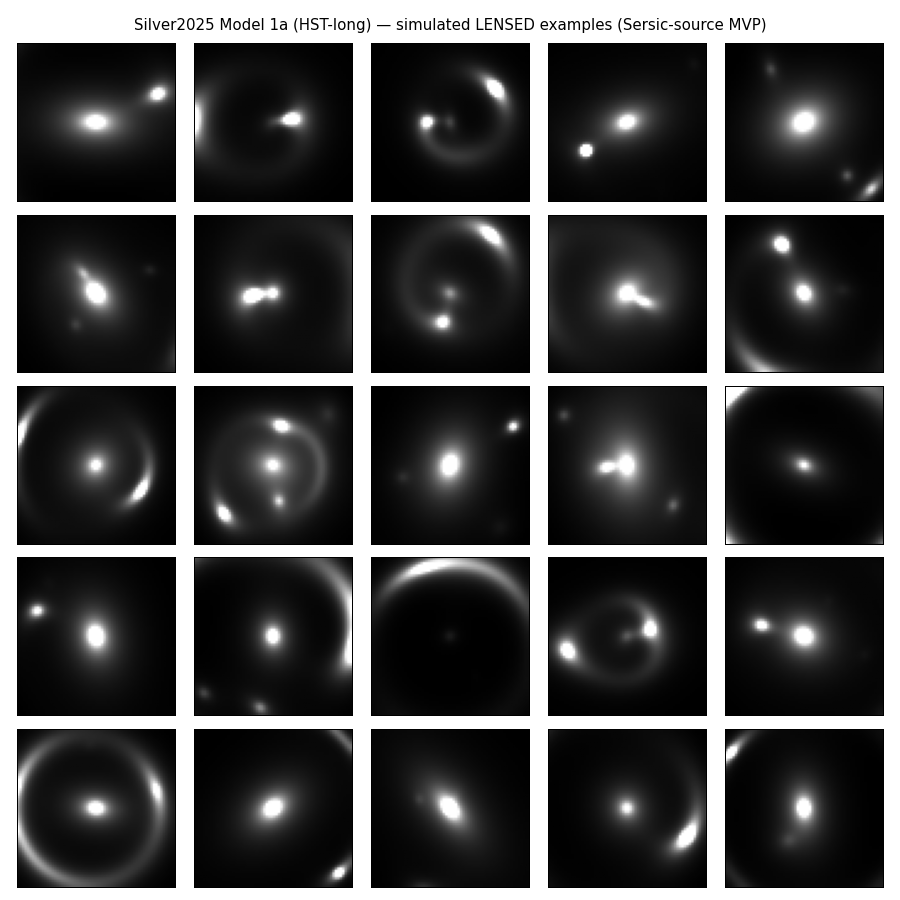
\includegraphics[width=\linewidth]{figures/sim_preview.png}\\[3pt]
  {\small\textbf{(a) This work (Fig.~\ref{fig:sims})}}
\end{minipage}\hfill
\begin{minipage}[b]{0.51\linewidth}\centering
  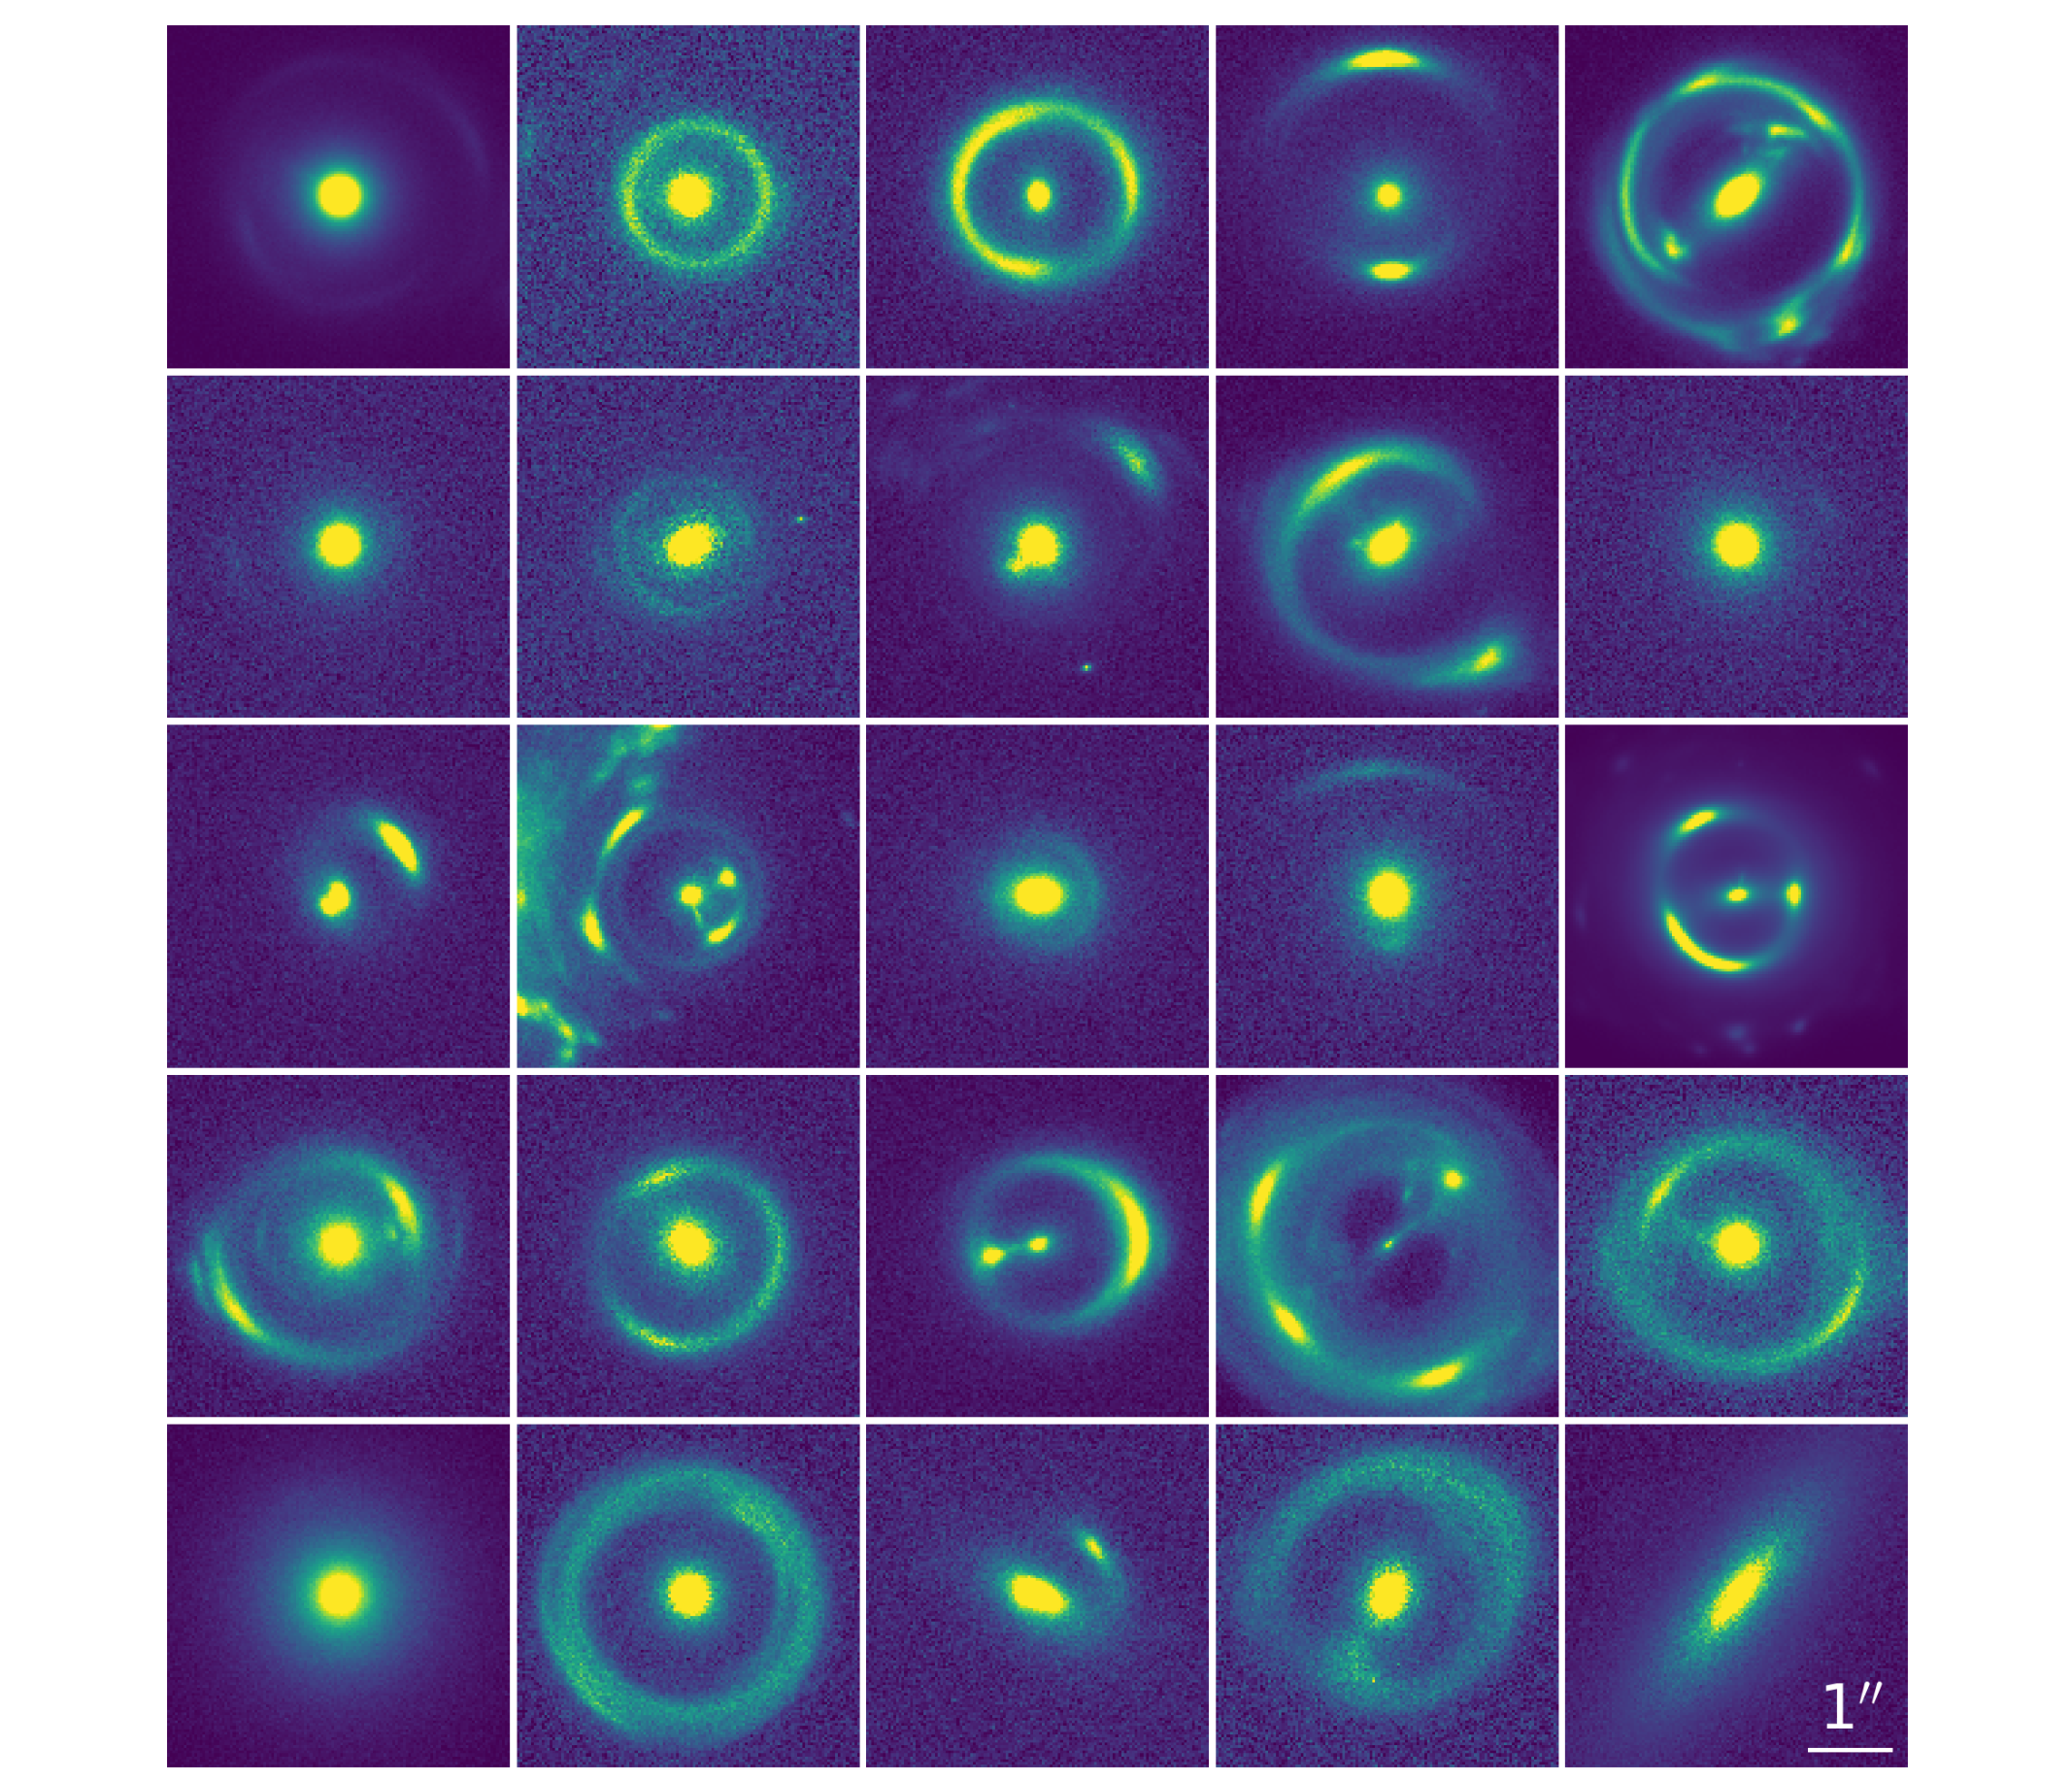
\includegraphics[width=\linewidth]{figures/orig_silver-2025_fig6.png}\\[3pt]
  {\small\textbf{(b) \citet{silver2025ml}, Fig.~6}}
\end{minipage}
\caption{\textbf{Simulated lensed Model~1a cutouts.} (a)~This work: 25
simulated \emph{lensed} cutouts ($64\times64$, $0.031''$/pixel, analytic
S\'ersic sources standing in for the paper's VELA stamps). (b)~The published
examples of simulated lensed systems with $0.5'' < \thetaE < 1.5''$ (Model~1,
HST). Both panels render the same conventional-lens morphology --- complete
Einstein rings, partial arcs, doubles, and quads. Panel (b) reproduced from
\citet{silver2025ml}, their Fig.~6, for comparison.}
\label{fig:cmp-silver-2025-sims}
\end{figure}

\begin{figure}[ht]
\centering
\begin{minipage}[b]{0.50\linewidth}\centering
  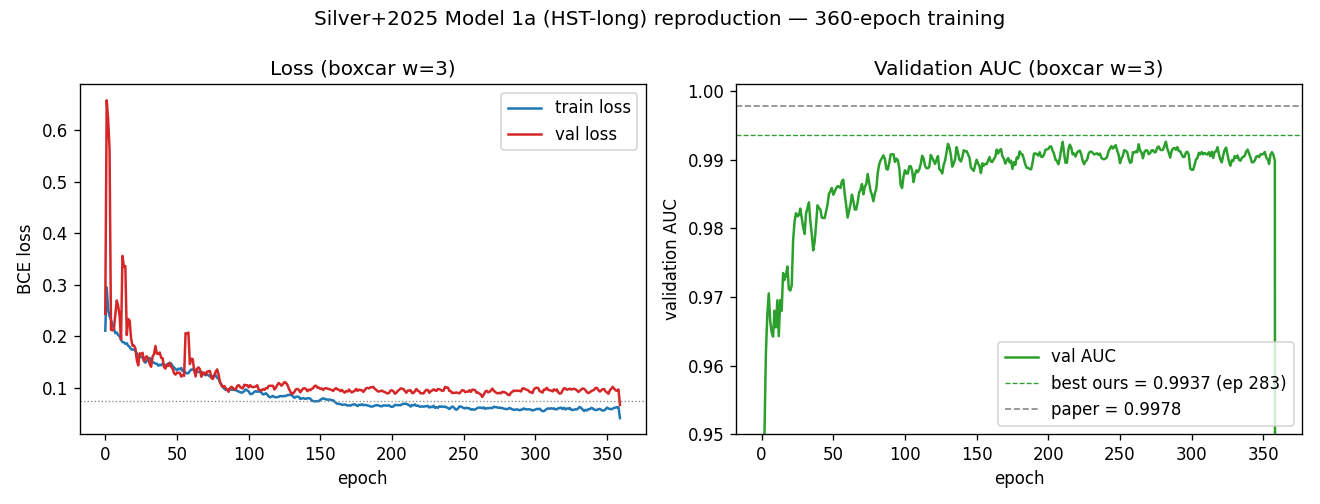
\includegraphics[width=\linewidth]{figures/training_curves_model1a.png}\\[3pt]
  {\small\textbf{(a) This work (Fig.~\ref{fig:curves})}}
\end{minipage}\hfill
\begin{minipage}[b]{0.47\linewidth}\centering
  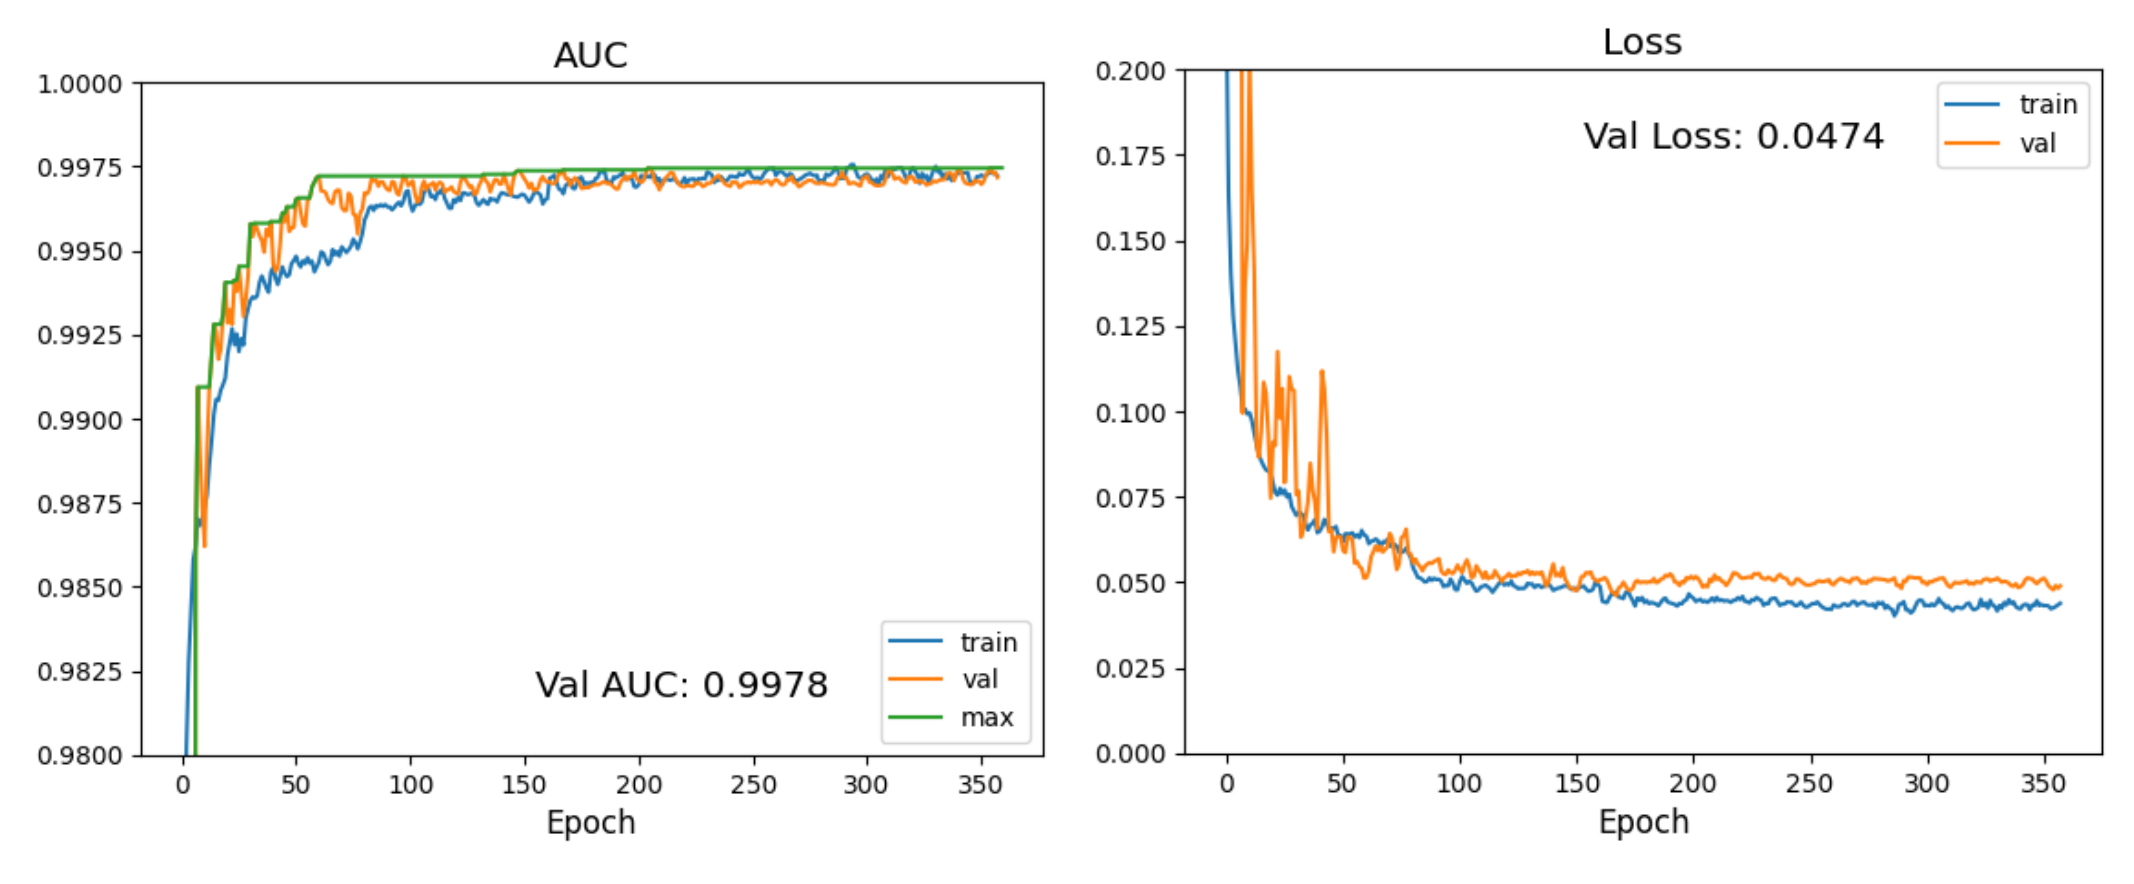
\includegraphics[width=\linewidth]{figures/orig_silver-2025_fig7.png}\\[3pt]
  {\small\textbf{(b) \citet{silver2025ml}, Fig.~7}}
\end{minipage}
\caption{\textbf{Model~1a training curves over 360 epochs.} (a)~This work:
train/validation BCE loss and validation AUC; our best $\mathrm{AUC} = 0.9937$
is reached at epoch~283 (boxcar-smoothed, window~3). (b)~The published loss and
AUC curves for Model~1a (HST-long), peak validation $\mathrm{AUC} = 0.9978$.
The two curves share the same shape --- AUC climbs past $0.99$ within the first
$\sim$80 epochs and plateaus near unity while the validation loss bottoms out
near $0.05$--$0.075$ --- and the peak values agree to within $0.4\,\%$. Panel
(b) reproduced from \citet{silver2025ml}, their Fig.~7, for comparison.}
\label{fig:cmp-silver-2025-curves}
\end{figure}

\begin{figure}[ht]
\centering
{\small\textbf{(a) This work (Table~\ref{tab:headline})}}\\[3pt]
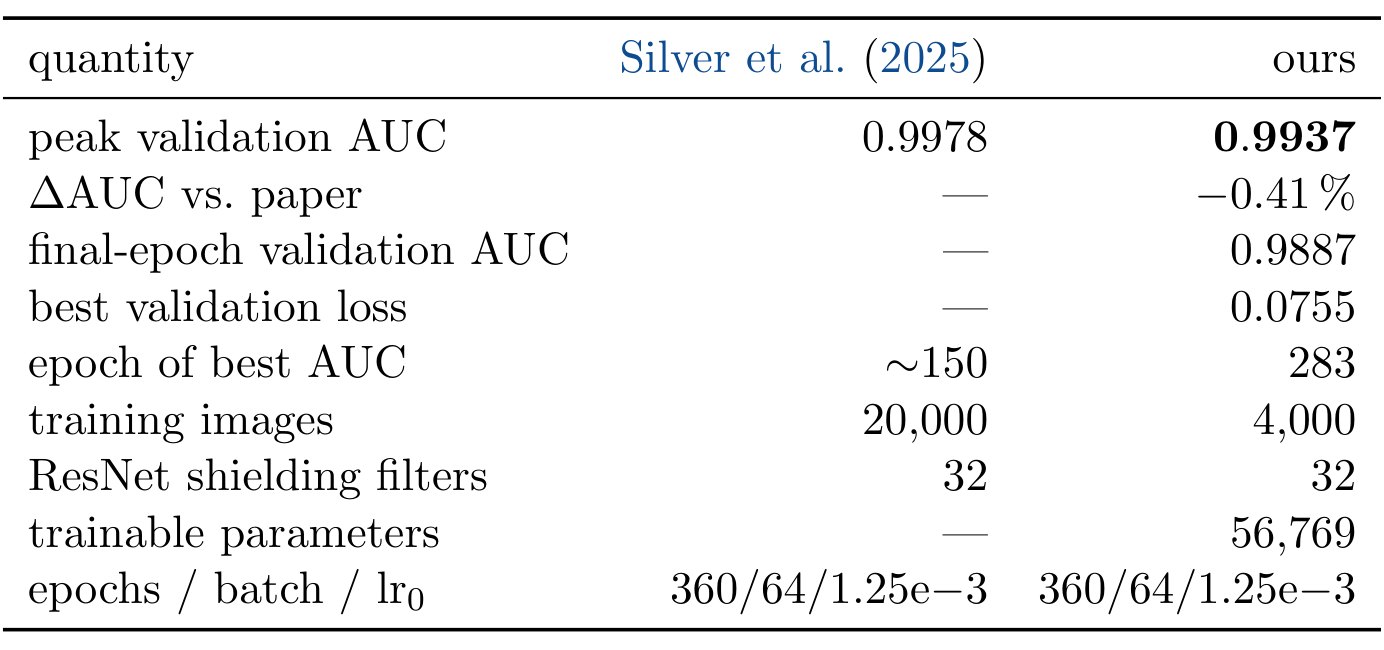
\includegraphics[width=0.72\linewidth]{figures/ours_silver-2025_tab_headline.png}\\[12pt]
{\small\textbf{(b) \citet{silver2025ml}, Table~3}}\\[3pt]
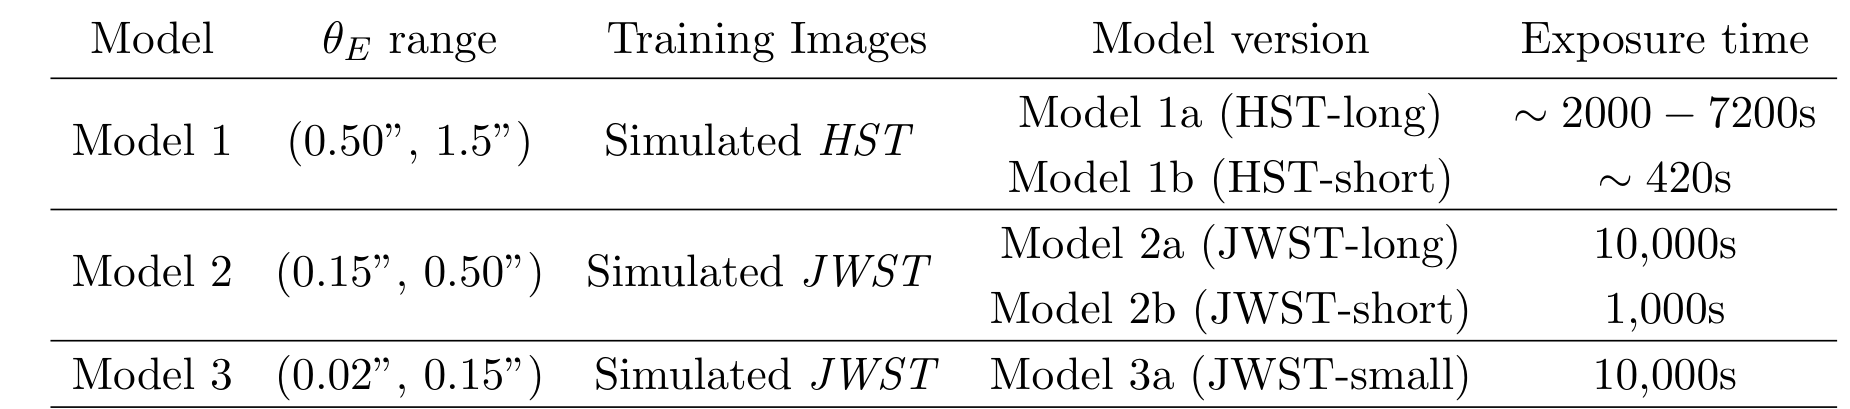
\includegraphics[width=0.92\linewidth]{figures/orig_silver-2025_table3.png}
\caption{\textbf{Model~1a definition and headline result.} (a)~This work
(Table~\ref{tab:headline}): our best validation $\mathrm{AUC} = 0.9937$ against
the published $0.9978$ (within $0.4\,\%$), with the matching training schedule
(360 epochs, batch~64, $\mathrm{lr}_0 = 1.25\times10^{-3}$, 32-filter shields).
(b)~The published ``Three ResNet Models'' table, which fixes the Model~1a
(HST-long) regime this reproduction targets --- $0.5'' < \thetaE < 1.5''$,
simulated HST, $\sim$2000--7200\,s exposures. The published peak AUC of
$0.9978$ itself is quoted in their Fig.~7 caption (\S3.2.1.1) rather than in
this table. Panel (b) reproduced from \citet{silver2025ml}, their Table~3, for
comparison.}
\label{fig:cmp-silver-2025-headline}
\end{figure}

\bibliographystyle{plainnat}
\bibliography{references}

\end{document}
